\documentclass[tikz,border=10pt]{standalone}
\usepackage{amsmath}
\usetikzlibrary{arrows.meta, positioning, calc, decorations.pathreplacing}
\definecolor{c1}{HTML}{000000}
\definecolor{c2}{HTML}{233D4D}
\definecolor{c3}{HTML}{FE7F2D}
\definecolor{c4}{HTML}{EAECF0}
\definecolor{axiscolor}{HTML}{333333}
\definecolor{labelcolor}{HTML}{5F6B75}
\begin{document}
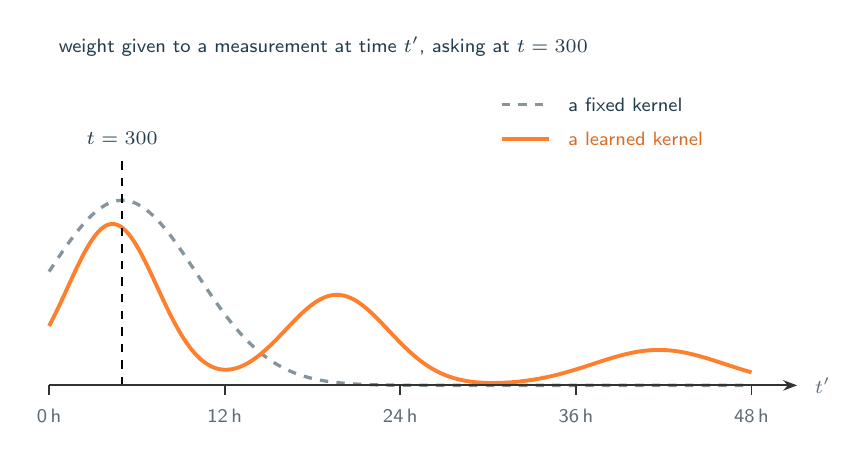
\begin{tikzpicture}[
    every node/.style={font=\sffamily},
    lab/.style={font=\sffamily\scriptsize, text=labelcolor},
    tag/.style={font=\sffamily\scriptsize, text=c2},
    hot/.style={font=\sffamily\scriptsize, text=c3!85!black},
]
\def\X#1{1.55 + #1*0.003100}

\node[tag, anchor=west] at (1.55, 5.45) {weight given to a measurement at time $t'$, asking at $t = 300$};

% a fixed RBF kernel
\draw[c2!55, line width=1.2pt, dashed]
    plot[domain=0:2880, samples=260, smooth]
    ({\X{\x}}, {1.15 + 2.35*exp(-((\x-300)/430)*((\x-300)/430))});


% a learned kernel: asymmetric, with a second lobe
\draw[c3, line width=1.4pt]
    plot[domain=0:2880, samples=320, smooth]
    ({\X{\x}}, {1.15 + 2.05*exp(-((\x-260)/260)*((\x-260)/260))
              + 1.15*exp(-((\x-1180)/300)*((\x-1180)/300))
              + 0.45*exp(-((\x-2500)/380)*((\x-2500)/380))});


\draw[c1, line width=0.8pt, dashed] ({\X{300}}, 1.15) -- ({\X{300}}, 4.05);
\node[tag, anchor=south] at ({\X{300}}, 4.09) {$t = 300$};

% legend
\draw[c2!55, line width=1.2pt, dashed] (7.30, 4.72) -- (7.90, 4.72);
\node[tag, anchor=west] at (8.02, 4.72) {a fixed kernel};
\draw[c3, line width=1.4pt] (7.30, 4.28) -- (7.90, 4.28);
\node[hot, anchor=west] at (8.02, 4.28) {a learned kernel};

\draw[axiscolor, line width=0.8pt, -{Stealth[length=5pt]}] (1.55, 1.15) -- (11.05, 1.15);
\foreach \h in {0, 12, 24, 36, 48}{
    \pgfmathsetmacro\m{\h*60}
    \draw[axiscolor, line width=0.7pt] ({\X{\m}}, 1.15) -- ({\X{\m}}, 1.03);
    \node[lab, anchor=north] at ({\X{\m}}, 0.97) {\h\,h};
}
\node[lab, anchor=west] at (11.15, 1.15) {$t'$};
\end{tikzpicture}
\end{document}
